\chapter{Исследовательская часть}

\section{Технические характеристики}

Технические характеристики устройства, на котором выполнялись замеры по времени, представлены далее.

\begin{enumerate}
	\item Процессор	Intel(R) Core(TM) i7-9750H CPU @ 2.60GHz, 2592 МГц, ядер: 6, логических процессоров: 12.
	\item Оперативная память: 16 ГБайт.
	\item Операционная система: Майкрософт Windows 10 Pro.
\end{enumerate}

При замерах времени ноутбук был включен в сеть электропитания и был нагружен только системными приложениями.

\section{Демонстрация работы программы}

На рисунке \ref{img:demonstration} представлена демонстрация работы разработанного программного обеспечения, 
показаны результаты вычислений расстояний Дамерау--Левенштейна и Левенштейна между словами <<fds>>,<<asd>>, заметим
что в случае поднятого флага вывода матриц происходит вывод матриц, использованных в расчетах.
\clearpage
\begin{figure}[H]
	\centering
	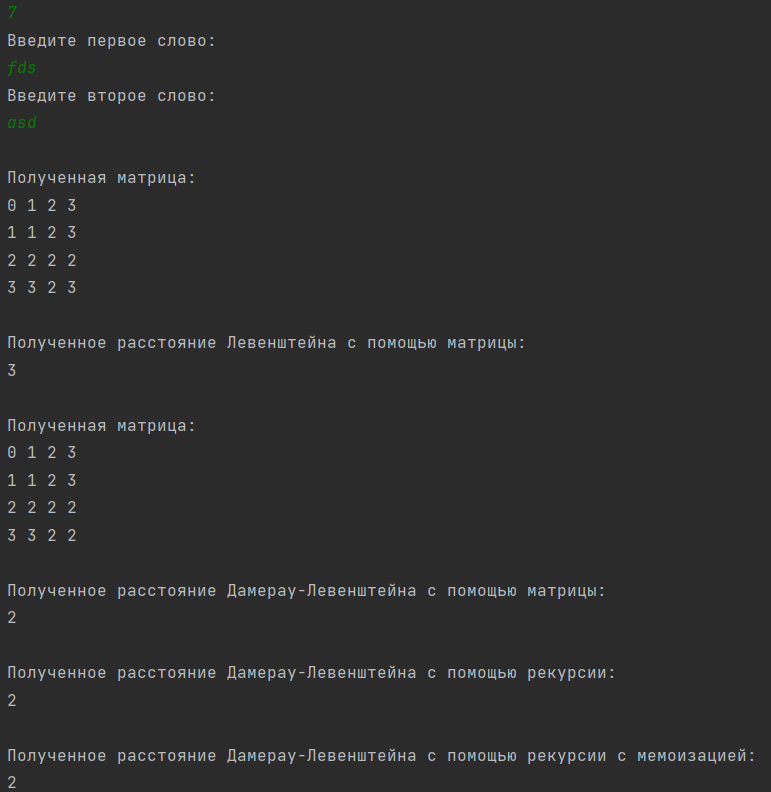
\includegraphics[height=0.7\textheight]{../img/programm_work.png}
	\caption{Демонстрация работы программы}
	\label{img:demonstration}
\end{figure}

\clearpage

\section{Временные характеристики}

Результаты эксперимента замеров по времени приведены в таблице \ref{t:timings}, каждый столбец таблице имеет заголовок в формате:
<<Алгоритм расчета-соответствующее расстояние>>, под <<Дамерау>> имеется в виду расстояние Дамерау--Левенштейна, под словом
<<Мемоизация>> имеется в виду  рекурсия с мемоизацией, описание которой приведено в разделе \ref{subec:memorysation_descr}.

Заметим, что некоторые поля в данной таблице
имеют значение <<->>, это обусловлено тем, что дальнейший расчет значений столбца <<Рекурсия-Дамерау>> окажется слишком
долгим, полученных данных достаточно для проведения исследования.

Замеры проводились на одинаковых длин строк от 1 до 100 с шагом 1, для получения достоверных результатов замеры 
времени для каждой пары строк проводились 100 раз, после чего усреднялись. Все результаты вычислений приведены в миллисекундах.


\begin{tiny}
    \begin{longtable}{|l|l|l|l|l|}
        \caption{Полученная таблица временных замеров различных реализаций поиска редакционных расстояний}\\
        \label{t:timings}\\
        \hline
        Длина слова & Матрица-Дамерау & Рекурсия-Дамерау & Мемоизация-Дамерау & Матрица-Левенштейн \\ \hline
        1 & 0.00134 & 0.00113 & 0.00126 & 0.00688 \\ \hline
        2 & 0.0014 & 0.00133 & 0.00156 & 0.00135 \\ \hline
        3 & 0.00172 & 0.0021 & 0.00194 & 0.00158 \\ \hline
        4 & 0.00214 & 0.00583 & 0.00408 & 0.00206 \\ \hline
        5 & 0.00262 & 0.02679 & 0.00322 & 0.00249 \\ \hline
        6 & 0.00466 & 0.13082 & 0.00419 & 0.00306 \\ \hline
        7 & 0.0028 & 0.48749 & 0.00346 & 0.00352 \\ \hline
        8 & 0.00301 & 2.3975 & 0.00494 & 0.00286 \\ \hline
        9 & 0.00457 & 13.881 & 0.00517 & 0.00425 \\ \hline
        10 & 0.0046 & 74.181 & 0.00657 & 0.00422 \\ \hline
        11 & 0.00523 & 416.8 & 0.0074 & 0.00476 \\ \hline
        12 & 0.0063 & 2423.0 & 0.00881 & 0.00569 \\ \hline
        13 & 0.00632 & - & 0.00876 & 0.00575 \\ \hline
        14 & 0.00854 & - & 0.00999 & 0.00658 \\ \hline
        15 & 0.00824 & - & 0.0115 & 0.0075 \\ \hline
        16 & 0.00909 & - & 0.01305 & 0.00923 \\ \hline
        17 & 0.01041 & - & 0.01559 & 0.00956 \\ \hline
        18 & 0.01202 & - & 0.016 & 0.01014 \\ \hline
        19 & 0.0126 & - & 0.01818 & 0.01148 \\ \hline
        20 & 0.01339 & - & 0.01958 & 0.0122 \\ \hline
        21 & 0.01464 & - & 0.02243 & 0.01338 \\ \hline
        22 & 0.01753 & - & 0.02401 & 0.01522 \\ \hline
        23 & 0.01769 & - & 0.02708 & 0.016 \\ \hline
        24 & 0.01889 & - & 0.02867 & 0.01709 \\ \hline
        25 & 0.02133 & - & 0.03004 & 0.01849 \\ \hline
        26 & 0.02241 & - & 0.03286 & 0.02148 \\ \hline
        27 & 0.02427 & - & 0.03635 & 0.02216 \\ \hline
        28 & 0.02539 & - & 0.03736 & 0.02485 \\ \hline
        29 & 0.0272 & - & 0.04016 & 0.02652 \\ \hline
        30 & 0.02931 & - & 0.04404 & 0.02675 \\ \hline
        31 & 0.03108 & - & 0.04581 & 0.02993 \\ \hline
        32 & 0.03355 & - & 0.05012 & 0.03049 \\ \hline
        33 & 0.03501 & - & 0.05191 & 0.03281 \\ \hline
        34 & 0.0407 & - & 0.05685 & 0.03382 \\ \hline
        35 & 0.03886 & - & 0.05863 & 0.03544 \\ \hline
        36 & 0.04309 & - & 0.06307 & 0.03907 \\ \hline
        37 & 0.04323 & - & 0.06525 & 0.03922 \\ \hline
        38 & 0.04734 & - & 0.07587 & 0.04526 \\ \hline
        39 & 0.05079 & - & 0.07475 & 0.04505 \\ \hline
        40 & 0.0554 & - & 0.08139 & 0.04885 \\ \hline
        41 & 0.05543 & - & 0.08094 & 0.05126 \\ \hline
        42 & 0.05758 & - & 0.09296 & 0.05472 \\ \hline
        43 & 0.05906 & - & 0.09024 & 0.05349 \\ \hline
        44 & 0.06341 & - & 0.09139 & 0.05691 \\ \hline
        45 & 0.06622 & - & 0.09554 & 0.05951 \\ \hline
        46 & 0.068 & - & 0.10273 & 0.06117 \\ \hline
        47 & 0.0712 & - & 0.10483 & 0.06496 \\ \hline
        48 & 0.07377 & - & 0.11548 & 0.06771 \\ \hline
        49 & 0.07676 & - & 0.11508 & 0.06909 \\ \hline
        50 & 0.0806 & - & 0.11882 & 0.07561 \\ \hline
        51 & 0.08402 & - & 0.12272 & 0.0767 \\ \hline
        52 & 0.08809 & - & 0.12774 & 0.07858 \\ \hline
        53 & 0.09262 & - & 0.13187 & 0.08221 \\ \hline
        54 & 0.09183 & - & 0.13909 & 0.08462 \\ \hline
        55 & 0.09647 & - & 0.14234 & 0.08714 \\ \hline
        56 & 0.1006 & - & 0.14796 & 0.09048 \\ \hline
        57 & 0.1028 & - & 0.15549 & 0.09485 \\ \hline
        58 & 0.10585 & - & 0.16104 & 0.09738 \\ \hline
        59 & 0.10826 & - & 0.16298 & 0.10099 \\ \hline
        60 & 0.11546 & - & 0.16882 & 0.10566 \\ \hline
        61 & 0.12044 & - & 0.17882 & 0.10939 \\ \hline
        62 & 0.12153 & - & 0.1808 & 0.11003 \\ \hline
        63 & 0.12612 & - & 0.18707 & 0.11303 \\ \hline
        64 & 0.129 & - & 0.19677 & 0.11822 \\ \hline
        65 & 0.1343 & - & 0.19808 & 0.13005 \\ \hline
        66 & 0.14127 & - & 0.21004 & 0.1253 \\ \hline
        67 & 0.14692 & - & 0.20936 & 0.13454 \\ \hline
        68 & 0.1679 & - & 0.22829 & 0.14849 \\ \hline
        69 & 0.15841 & - & 0.22867 & 0.14192 \\ \hline
        70 & 0.15921 & - & 0.24836 & 0.14623 \\ \hline
        71 & 0.15988 & - & 0.2375 & 0.14523 \\ \hline
        72 & 0.16827 & - & 0.24643 & 0.15342 \\ \hline
        73 & 0.17037 & - & 0.25365 & 0.156 \\ \hline
        74 & 0.17445 & - & 0.26027 & 0.15706 \\ \hline
        75 & 0.1839 & - & 0.26633 & 0.16341 \\ \hline
        76 & 0.18451 & - & 0.2745 & 0.16571 \\ \hline
        77 & 0.19255 & - & 0.28234 & 0.17876 \\ \hline
        78 & 0.19624 & - & 0.28753 & 0.17891 \\ \hline
        79 & 0.20694 & - & 0.29764 & 0.18215 \\ \hline
        80 & 0.20866 & - & 0.30539 & 0.18861 \\ \hline
        81 & 0.20868 & - & 0.31365 & 0.18863 \\ \hline
        82 & 0.21407 & - & 0.32003 & 0.19693 \\ \hline
        83 & 0.22075 & - & 0.32734 & 0.20323 \\ \hline
        84 & 0.25258 & - & 0.34314 & 0.20608 \\ \hline
        85 & 0.23223 & - & 0.34761 & 0.20881 \\ \hline
        86 & 0.23893 & - & 0.36106 & 0.21708 \\ \hline
        87 & 0.25343 & - & 0.37841 & 0.23564 \\ \hline
        88 & 0.26672 & - & 0.3987 & 0.23541 \\ \hline
        89 & 0.2565 & - & 0.37914 & 0.22846 \\ \hline
        90 & 0.25403 & - & 0.39294 & 0.25183 \\ \hline
        91 & 0.26909 & - & 0.39794 & 0.24198 \\ \hline
        92 & 0.27941 & - & 0.39998 & 0.24435 \\ \hline
        93 & 0.28903 & - & 0.42276 & 0.25272 \\ \hline
        94 & 0.28921 & - & 0.43863 & 0.26984 \\ \hline
        95 & 0.31258 & - & 0.45226 & 0.28118 \\ \hline
        96 & 0.31653 & - & 0.46734 & 0.28617 \\ \hline
        97 & 0.32134 & - & 0.47819 & 0.28236 \\ \hline
        98 & 0.30153 & - & 0.45308 & 0.27619 \\ \hline
        99 & 0.31551 & - & 0.47476 & 0.30401 \\ \hline
        100 & 0.46852 & - & 0.61734 & 0.38562 \\ \hline
    \end{longtable}
\end{tiny}

Имеет смысл сравнить поиск расстояний Левенштейна и Дамерау--Левенштейна при использовании матрицы. Заметим, что при использовании
алгоритма поиска расстояния Дамерау--Левенштейна, при рассмотрении слов длины больше 80 затрачивается больше времени, чем 
при использоавнии алгоритма Левенштейна. Данная закономерность обусловлена дополнительной операцией обмена символов, которую 
необходимо учитывать при поиске расстояния Дамерау-Левенштейна. Графики \ref{plt:time_matrix_cmp, plt:time_mat_rec_cmp, plt:time_rec_cmp} получены при 
помощи анализа данных таблицы \ref{t:timings}.

\begin{figure}[h]
	\centering
	\includesvg[height=0.3\textheight]{../img/matrixCmp.svg}
	\caption{Сравнение по времени нерекурсивных реализаций алгоритмов поиска расстояний Левенштейна и Дамерау-Левенштейна}
	\label{plt:time_matrix_cmp}
\end{figure}

Также необходимо сравнить реализации рекурсивного поиска расстояния Дамерау-Левенштейна с мемоизацией и без, полученный график приведен
на картинке \ref{plt:time_rec_cmp}. Заметим, что рекурсия с мемоизацией, засчет сохранения информации о уже расчитанных расстояниях подстрок
показала себя заметно эффективнее, чем рекурсия без мемоизации. 


\begin{figure}[h]
	\centering
	\includesvg[height=0.3\textheight]{../img/recCmp.svg}
	\caption{Сравнение по времени реализации рекурсивного поиска расстояния Дамерау-Левенштейна с мемоизацией и без}
	\label{plt:time_rec_cmp}
\end{figure}

Стоит отметить, что при сравнении реализации рекурсивного поиска расстояния Дамерау-Левенштейна с  мемоизацией и поиска
с использованием матрицы (см. \ref{plt:time_mat_rec_cmp}), реализация с использованием матрицы показала себя более эффективной
по времени. 

\begin{figure}[h]
	\centering
	\includesvg[height=0.3\textheight]{../img/matRecCmp.svg}
	\caption{Сравнение по времени реализации рекурсивного поиска расстояния Дамерау-Левенштейна с  мемоизацией, с поиском
	расстояния с использоавнием матрицы}
	\label{plt:time_mat_rec_cmp}
\end{figure}


\section{Характеристики по памяти}

Введем следующие обозначения:
\begin{enumerate}
	\item $size_{1}$ --- длина строки $S_{1}$.
	\item $size_{2}$ --- длина строки $S_{2}$,
	\item $sizeof$ --- функция вычисляющая размер в байтах.
	\item $wstring$ --- строковый тип.
	\item $wstring\&$ --- указатель на строковый тип.
	\item $matrix\&$ --- указатель на матрицу.
	\item $int$ --- целочисленный тип.
	\item $size\_t$ --- беззнаковый целочисленный тип.
\end{enumerate}

Максимальная глубина стека вызовов при рекурсивной реализации нахождения расстояния Дамерау--Левенштейна равна сумме входящих строк,
так как дерево рекурсии будет расти пока длина хотя бы одной строки не будет равна 1. Таким образом при рекурсивном поиске данного расстояния затраченная память
будет рассчитываться  аналогично примеру \ref{eq:dl_rec_memory}.
\begin{equation}
	\label{eq:dl_rec_memory}
	(n + m) \cdot (2 \cdot sizeof(wstring\&) + sizeof(int) + 6 \cdot sizeof(size\_t)) +  (2 \cdot sizeof(wstring))
\end{equation}
где:
\begin{itemize}
	\item $2 \cdot sizeof(string)$ --- хранение двух строк;
	\item $2 \cdot sizeof(int)$ --- хранение размеров рассматриваемых подстрок;
	\item $2 \cdot sizeof(string\&)$ --- хранение указателей на строки;
	\item $6 \cdot sizeof(size\_t)$ --- вспомогательные переменные;
	\item $sizeof(int)$ --- адрес возврата.
\end{itemize}

Заметим, что в данном случае считается, что в типе $string$ хранятся все необходимые данные для задания строки(т.е. $size + 1$ символ).

Для рекурсивного алгоритма c кешированием поиска расстояния Дамерау-Левенштейна будет теоретически схож с расчетом в формуле (\ref{eq:dl_rec_memory}),
но также учитывается матрица, соответственно, максимальный расход памяти равен:
\begin{equation}
	\label{eq:dl_hash_memory}
    \small
	\begin{aligned}
		(n + m) \cdot (2 \cdot sizeof(string\&) + sizeof(int) + sizeof(matrix\&) + 6 \cdot sizeof(size\_t)) \\
        + (2 \cdot sizeof(string) + sizeof(matrix))
	\end{aligned}
\end{equation}

Затраты памяти на хранение матрицы описаны в  \ref{eq:matrix_mem}.
\begin{equation}
	\label{eq:matrix_mem}
    \begin{align}
	sizeof(matrix) = sizeof(int) \cdot (n+1) \cdot (m + 1)  \\
    + sizeof(int) \cdot 2 + sizeof(int\&) \cdot (n + 1) + sizeof(int\&\&).
    \end{align}
\end{equation}
В данном случае считается, что:
\begin{itemize}
	\item $sizeof(int) \cdot (n+1) \cdot (m + 1)$ --- хранение данных матрицы;
	\item $sizeof(int) \cdot 2$ --- хранение размеров матрицы;
	\item $sizeof(int\&) \cdot (n + 1)$ --- хранение строк матрицы;
	\item $sizeof(int\&\&)$ --- хранение указателя на матрицу;
\end{itemize}


Использование памяти при итеративной реализации алгоритма поиска расстояния левенштейна теоретически равно:
\begin{equation}
	\label{eq:lev_mtr_memory}
	\begin{aligned}
		sizeof(matrix) + sizeof(matrix&) + 2 \cdot sizeof(wstring\&)\\
        + 2 \cdot sizeof(wstring&) + sizeof(int) + 3 \cdot sizeof(int).
	\end{aligned}
\end{equation}
где 
\begin{itemize}
	\item $sizeof(matrix) + sizeof(matrix\&)$ --- хранение матрицы и ее указателя в кадре стека;
	\item $2 \cdot sizeof(wstring) + 2 \cdot sizeof(wstring)$ --- хранение строк и их указателей в кадре стека;
	\item $(n + 1) \cdot (m + 1) \cdot size(int)$ --- хранение матрицы;
	\item $3 \cdot sizeof(int)$ --- вспомогательные переменные.
	\item $sizeof(int)$ --- адрес возврата.
\end{itemize}

Использование памяти при итеративной реализации алгоритма поиска расстояния Дамерау--Левенштейна аналогично приведенному
в \ref{eq:lev_mtr_memory}.

По формулам \ref{eq:dl_rec_memory} -- \ref{eq:lev_mtr_memory} затрат по памяти в программе были написаны соответствующие функции для подсчета расходуемой памяти, результаты расчетов, которых представлены в таблице \ref{t:memory}, где размеры строк находятся в диапазоне от 10 до 200 с шагом 10.

\clearpage

\begin{table}[!ht]
    \centering
    \small
    \caption{Полученная таблица замеров по памяти различных реализаций поиска редакционных расстояний}
    \label{t:memory}
    \begin{tabular}{|l|l|l|l|l|}
    \hline
        Матрица-Левенштейн & Матрица-Дамерау & Рекурсия-Дамерау & Мемоизация-Дамерау & Матрица-Левенштейн \\ \hline
        0 & 200 & 64 & 132 & 200 \\ \hline
        10 & 760 & 2464 & 3652 & 760 \\ \hline
        20 & 2120 & 4864 & 7972 & 2120 \\ \hline
        30 & 4280 & 7264 & 13092 & 4280 \\ \hline
        40 & 7240 & 9664 & 19012 & 7240 \\ \hline
        50 & 11000 & 12064 & 25732 & 11000 \\ \hline
        60 & 15560 & 14464 & 33252 & 15560 \\ \hline
        70 & 20920 & 16864 & 41572 & 20920 \\ \hline
        80 & 27080 & 19264 & 50692 & 27080 \\ \hline
        90 & 34040 & 21664 & 60612 & 34040 \\ \hline
        100 & 41800 & 24064 & 71332 & 41800 \\ \hline
        110 & 50360 & 26464 & 82852 & 50360 \\ \hline
        120 & 59720 & 28864 & 95172 & 59720 \\ \hline
        130 & 69880 & 31264 & 108292 & 69880 \\ \hline
        140 & 80840 & 33664 & 122212 & 80840 \\ \hline
        150 & 92600 & 36064 & 136932 & 92600 \\ \hline
        160 & 105160 & 38464 & 152452 & 105160 \\ \hline
        170 & 118520 & 40864 & 168772 & 118520 \\ \hline
        180 & 132680 & 43264 & 185892 & 132680 \\ \hline
        190 & 147640 & 45664 & 203812 & 147640 \\ \hline
        200 & 163400 & 48064 & 222532 & 163400 \\ \hline
    \end{tabular}
\end{table}

Проанализировав таблицу \ref{t:memory}, можно сделать вывод, что по расходу памяти итеративные алгоритмы 
проигрывают рекурсивным: максимальный размер используемой памяти в итеративном растет как произведение длин строк,
в то время как у рекурсивного алгоритма — как сумма длин строк.

Также стоит отметить, что при малых длинах слов рекурсивные алгоритмы уступают итеративным, это обусловлено большим 
количеством вспомогательных переменных в реализации рекурсивного алгоритма.

\begin{figure}[H]
	\centering
	\includesvg[height=0.3\textheight]{../img/matRecCmpMem.svg}
	\caption{Сравнение по памяти алгоритмов поиска расстояния Левенштейна и Дамерау-Левенштейна --- итеративной и рекурсивной реализации}
	\label{plt:memory_mat_rec}
\end{figure}

Из рисунка \ref{plt:memory_mat_rec} понятно, что рекурсивная реализация алгоритма поиска расстояния Дамерау-Левенштейна эффективная по памяти, чем итеративная.

\begin{figure}[H]
	\centering
	\includesvg[height=0.3\textheight]{../img/recCmpMem.svg}
	\caption{Сравнение по памяти алгоритмов поиска расстояния Дамерау-Левенштейна --- рекурсивной реализации с мемоизацией и без}
	\label{plt:memory_rec}
\end{figure}

\clearpage

\section{Вывод}

В данном разделе было произведено сравнение количества затраченного времени и памяти алгоритмов поиска расстояний Левенштейна и Дамерау-Левенштейна. Наименее затратным по времени оказался итеративный алгоритм нахождения расстояния Левенштейна.
Наиболее эффективным по памяти оказалась рекурсивная реализация алгоритма поиска расстояния Дамерау-Левенштейна.
Рекурсивная реализация алгоритма поиска расстояния Дамерау-Левенштейна будет более затратным по времени по сравнению с итеративной реализацией алгоритма поиска расстояния Дамерау-Левенштейна, но менее затратным по памяти по отношению к итеративному алгоритму Дамерау-Левенштейна.
